\documentclass[a4paper]{ctexart}
\usepackage[utf8]{inputenc}
\usepackage[a4paper]{geometry}
\usepackage{graphicx}
\usepackage{float}
\usepackage{hyperref}
\usepackage[heading = false]{ctex}
\usepackage{xcolor}
\usepackage{fontspec}
\usepackage{listings}
\usepackage{color}

\definecolor{dkgreen}{rgb}{0,0.6,0}
\definecolor{gray}{rgb}{0.5,0.5,0.5}
\definecolor{mauve}{rgb}{0.58,0,0.82}

\lstset{frame=tb,
  aboveskip=3mm,
  belowskip=3mm,
  showstringspaces=false,
  columns=flexible,
  basicstyle={\small\ttfamily},
  numbers=none,
  numberstyle=\tiny\color{gray},
  keywordstyle=\color{blue},
  commentstyle=\color{dkgreen},
  stringstyle=\color{mauve},
  breaklines=true,
  breakatwhitespace=true,
  tabsize=3
}
\pagestyle{plain}
\geometry{top=1.0cm, bottom=2.0cm}
\lstset{
    basicstyle = \ttfamily,
    commentstyle = \itshape,
    % numbers = left,
    numberstyle = \zihao{-5}\ttfamily,
    % frame = lrtb
}

\begin{document}
  \begin{titlepage}
      \songti
      \begin{center}
        \vspace*{2cm}
        
\includegraphics[width=0.7\textwidth]{../HDU.png}\\
        \vspace*{1cm}
        {\fontsize{36pt}{0}
          \textbf{机器学习实验\\报\quad 告\\}
        }
        \vspace*{12cm}
        {\fontsize{18pt}{0}
          \makebox[80pt]{\textbf{实验名称}} \underline{\makebox[250pt]{\Large 手写数字识别}}\\
          \vspace*{0.5cm}
          \makebox[80pt]{\textbf{学\qquad 院}} \underline{\makebox[250pt]{\Large 通信工程学院}}\\
          \vspace*{0.5cm}
          \makebox[80pt]{\textbf{专\qquad 业}} \underline{\makebox[250pt]{\Large xxxx}}\\
          \vspace*{0.5cm}
          \makebox[80pt]{\textbf{学\qquad 号}} \underline{\makebox[250pt]{\Large xxxx}}\\
          \vspace*{0.5cm}
          \makebox[80pt]{\textbf{学生姓名}} \underline{\makebox[250pt]{\Large xxx}}\\
        }
      \end{center}
  \end{titlepage}

  \CTEXsetup[format={\Large\bfseries}]{section}

  \newpage
  \section{实验目的}
  \begin{enumerate}
    \item 理解图像识别、手写识别的原理
    \item 掌握Sklearn实现基于MLP的手写识别
    \item 掌握Sklearn实现基于KNN的手写识别
  \end{enumerate}

  \section{实验内容与要求}
  \begin{itemize}
    \item 手写数字识别是一个多分类问题,共有10个分类,每个手写数字图像
    的类别标签是0--9中的其中一个数。
    \item 利用sklearn来训练一个简单的全连接神经网络,即多层感知机(MLP),
    用于识别数据集DBRHD的手写数字。
    \item 利用sklearn来训练一个K最近临(KNN)分类器,用于识别数据集DBRHD的手写数字
    \item 比较MLP和KNN的识别效果
  \end{itemize}

  \section{实验程序与结果}
  \subsection{程序代码}
  \lstinputlisting[language=Python]{lab5.py}
  \subsection{运行结果}
  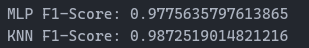
\includegraphics[width=0.5\textwidth]{fig/output.png}

  \newpage
  \section{实验结果分析}
  从结果可以看出,KNN的分类效果要略微好于MLP。
  但是由于MLP的超参数有很多,经过仔细调参后或许能达到优于KNN的分类效果。

  \section{实验问题解答与体会}
  本次实验使用了MLP和KNN完成了手写数字识别任务,让我对MLP和KNN有了更深的理解。

\end{document}
